\documentclass[11pt]{article}
\usepackage[margin=1in]{geometry}
\usepackage{graphicx}
\usepackage{hyperref}
\usepackage{xcolor}
\usepackage{parskip}

\definecolor{gold}{HTML}{C4A35A}

\title{\textcolor{gold}{Poetry Deep Looking}}
\author{Paul Fishwick and Claude Code}
\date{February 2026}

\begin{document}
\maketitle

\section{Overview}

Poetry Deep Looking is an interactive web application that pairs visual art with poetry. Users explore paintings by hovering over segmented regions, each of which reveals a contextually matched poem excerpt. The application uses AI-generated segmentation masks (via Google Gemini Pro) to map artwork regions to poems.

\section{Gallery}

The application opens with a gallery of artwork thumbnails. Each card shows the painting and its attribution. Clicking a card opens the interactive viewer.

\begin{figure}[h]
\centering
\includegraphics[width=0.85\textwidth]{gallery.png}
\caption{Gallery screen showing two artworks: \emph{Marsh Boardwalk North} by Stan Cottle and \emph{The Mouth of the Lourmarin River} by Paul Camille Guigou (1867).}
\label{fig:gallery}
\end{figure}

\section{Hover Interaction}

In the viewer, moving the cursor over a recognized region displays a popup with the poem title, poet name, a generated illustration, and a highlighted excerpt. The popup follows the cursor and updates as the user moves between regions.

\begin{figure}[h]
\centering
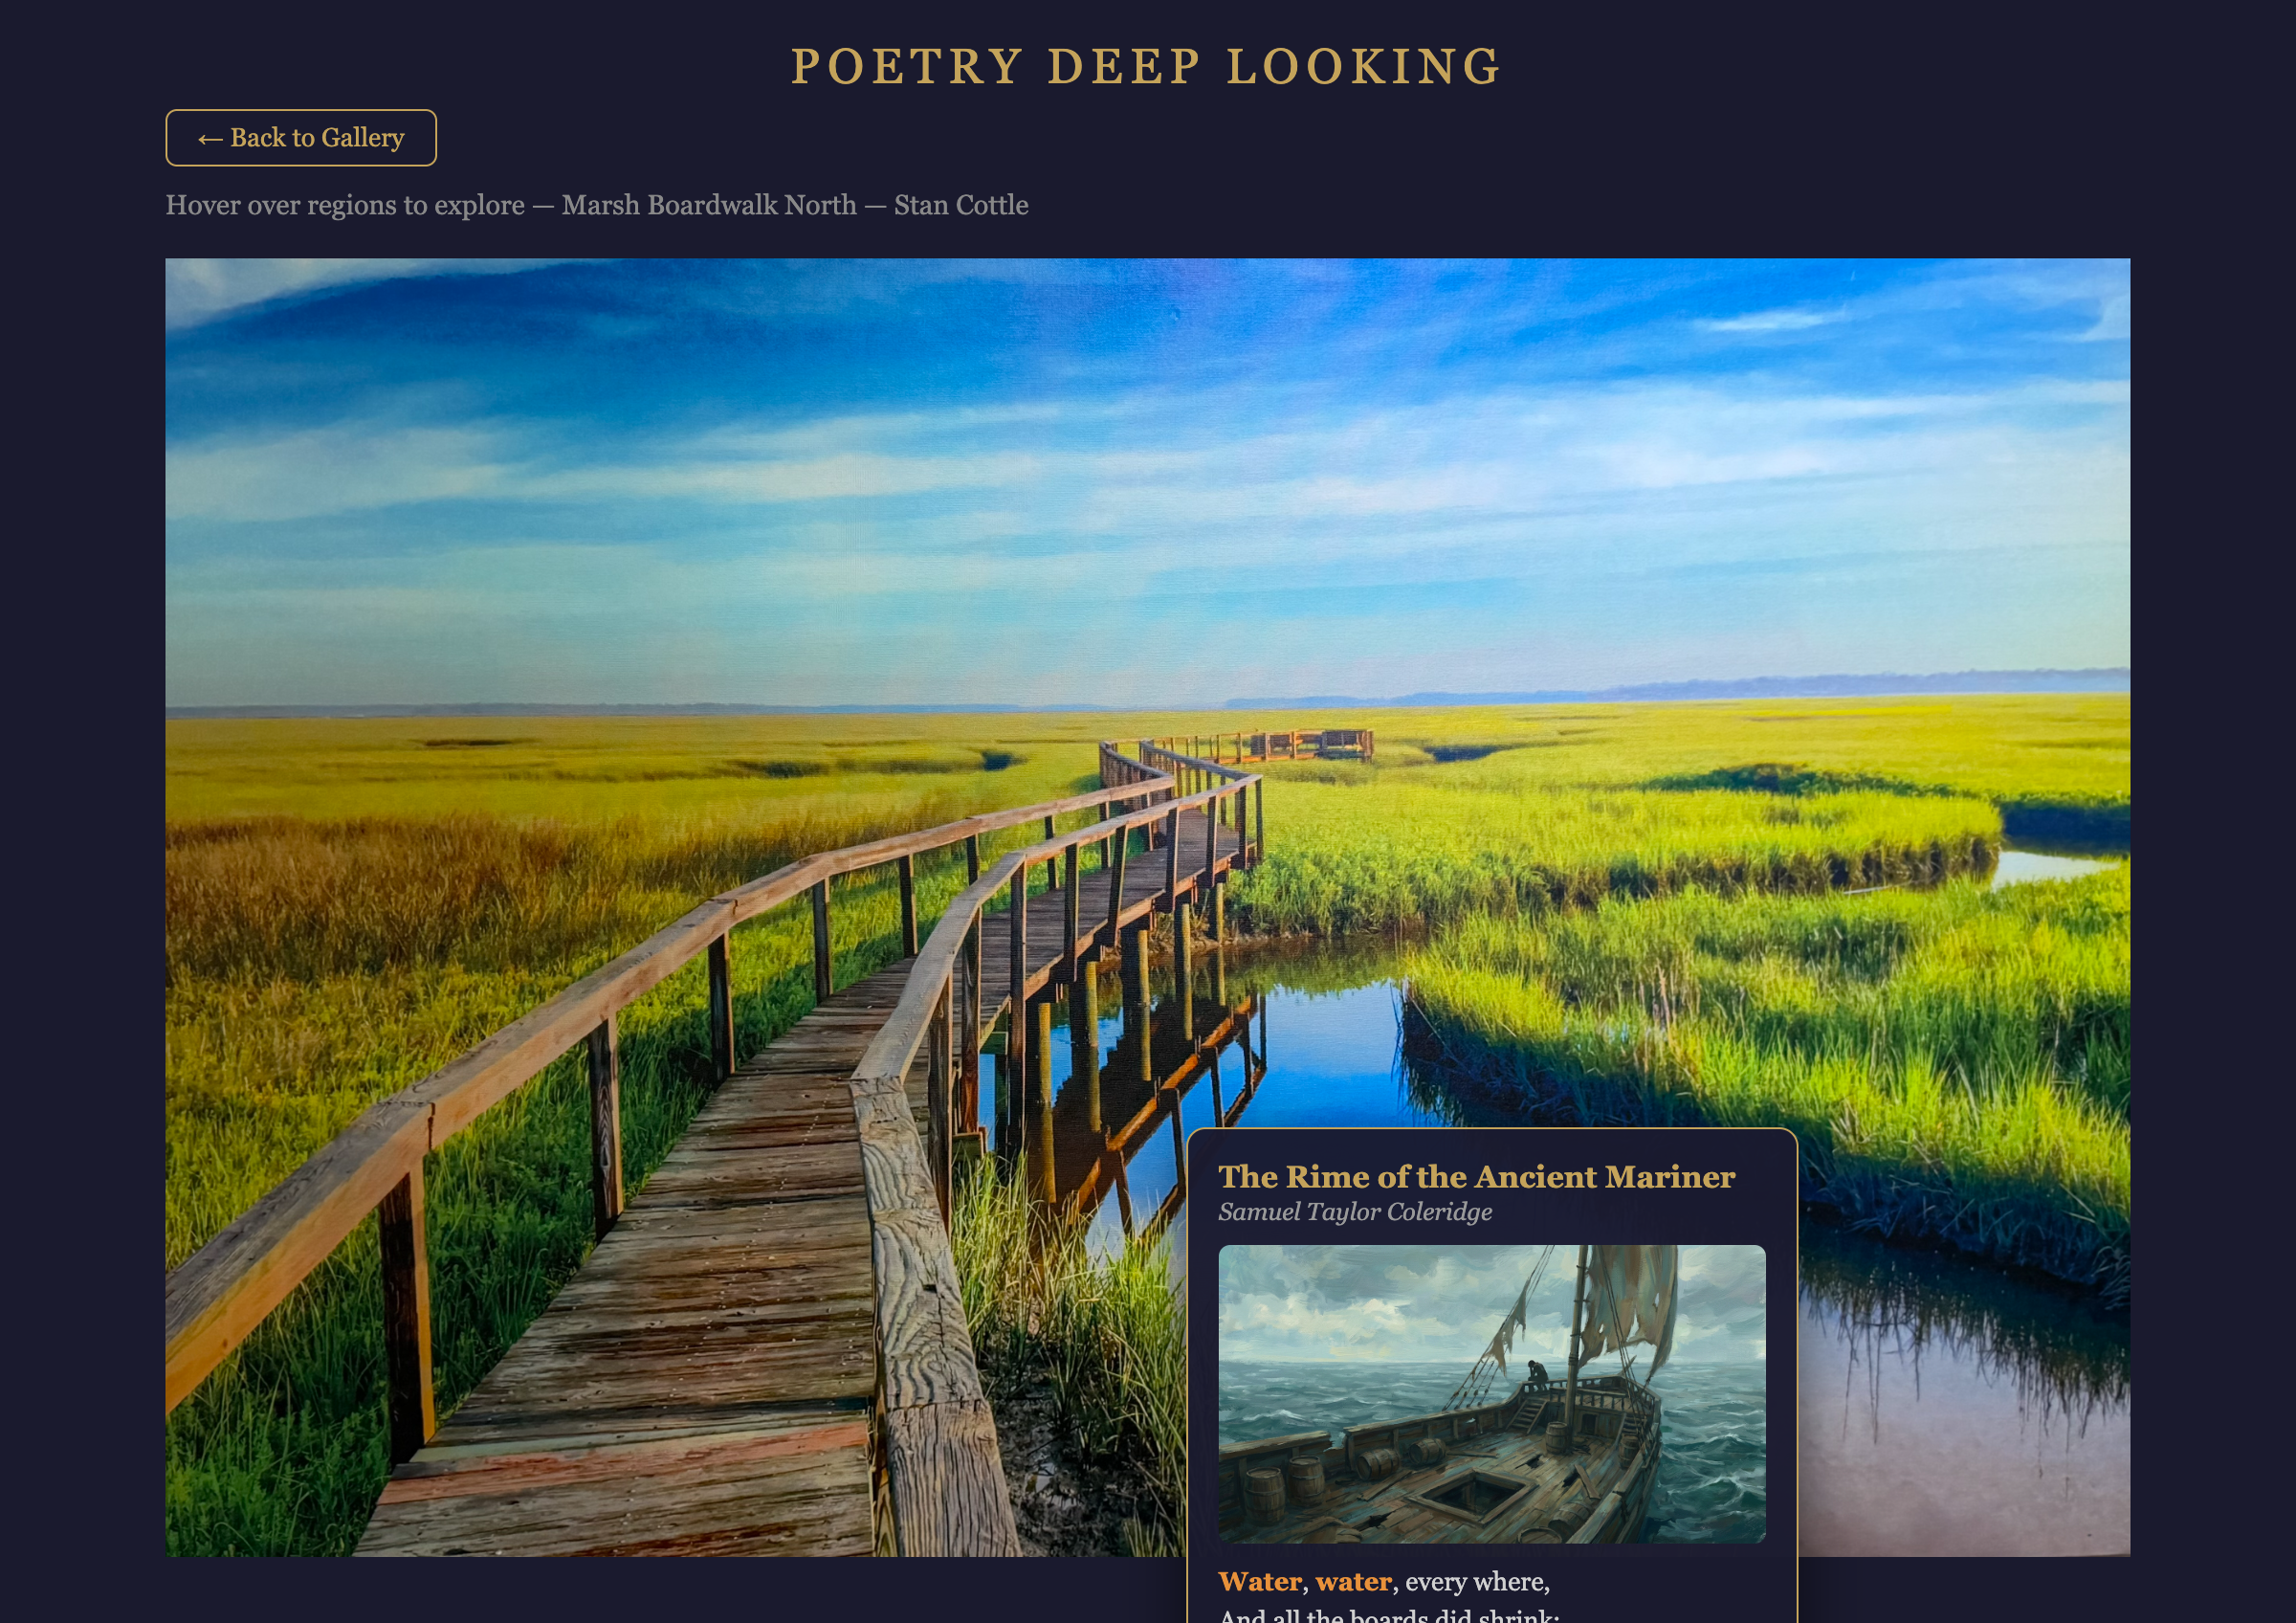
\includegraphics[width=0.85\textwidth]{hover-popup.png}
\caption{Hovering over the tidal creek in the Marsh painting reveals \emph{The Rime of the Ancient Mariner} by Samuel Taylor Coleridge.}
\label{fig:hover}
\end{figure}

\section{Click-to-Freeze Popup}

Clicking while a popup is visible pins it in place. The pinned popup displays a close button (\textsf{X}) in the top-right corner and converts the poem title into a hyperlink that opens the full poem in a new browser tab.

\begin{figure}[h]
\centering
\includegraphics[width=0.85\textwidth]{pinned-popup.png}
\caption{Pinned popup on the Marsh painting. The \textsf{X} button is visible and the title is now a clickable link to the full poem.}
\label{fig:pinned}
\end{figure}

\begin{figure}[h]
\centering
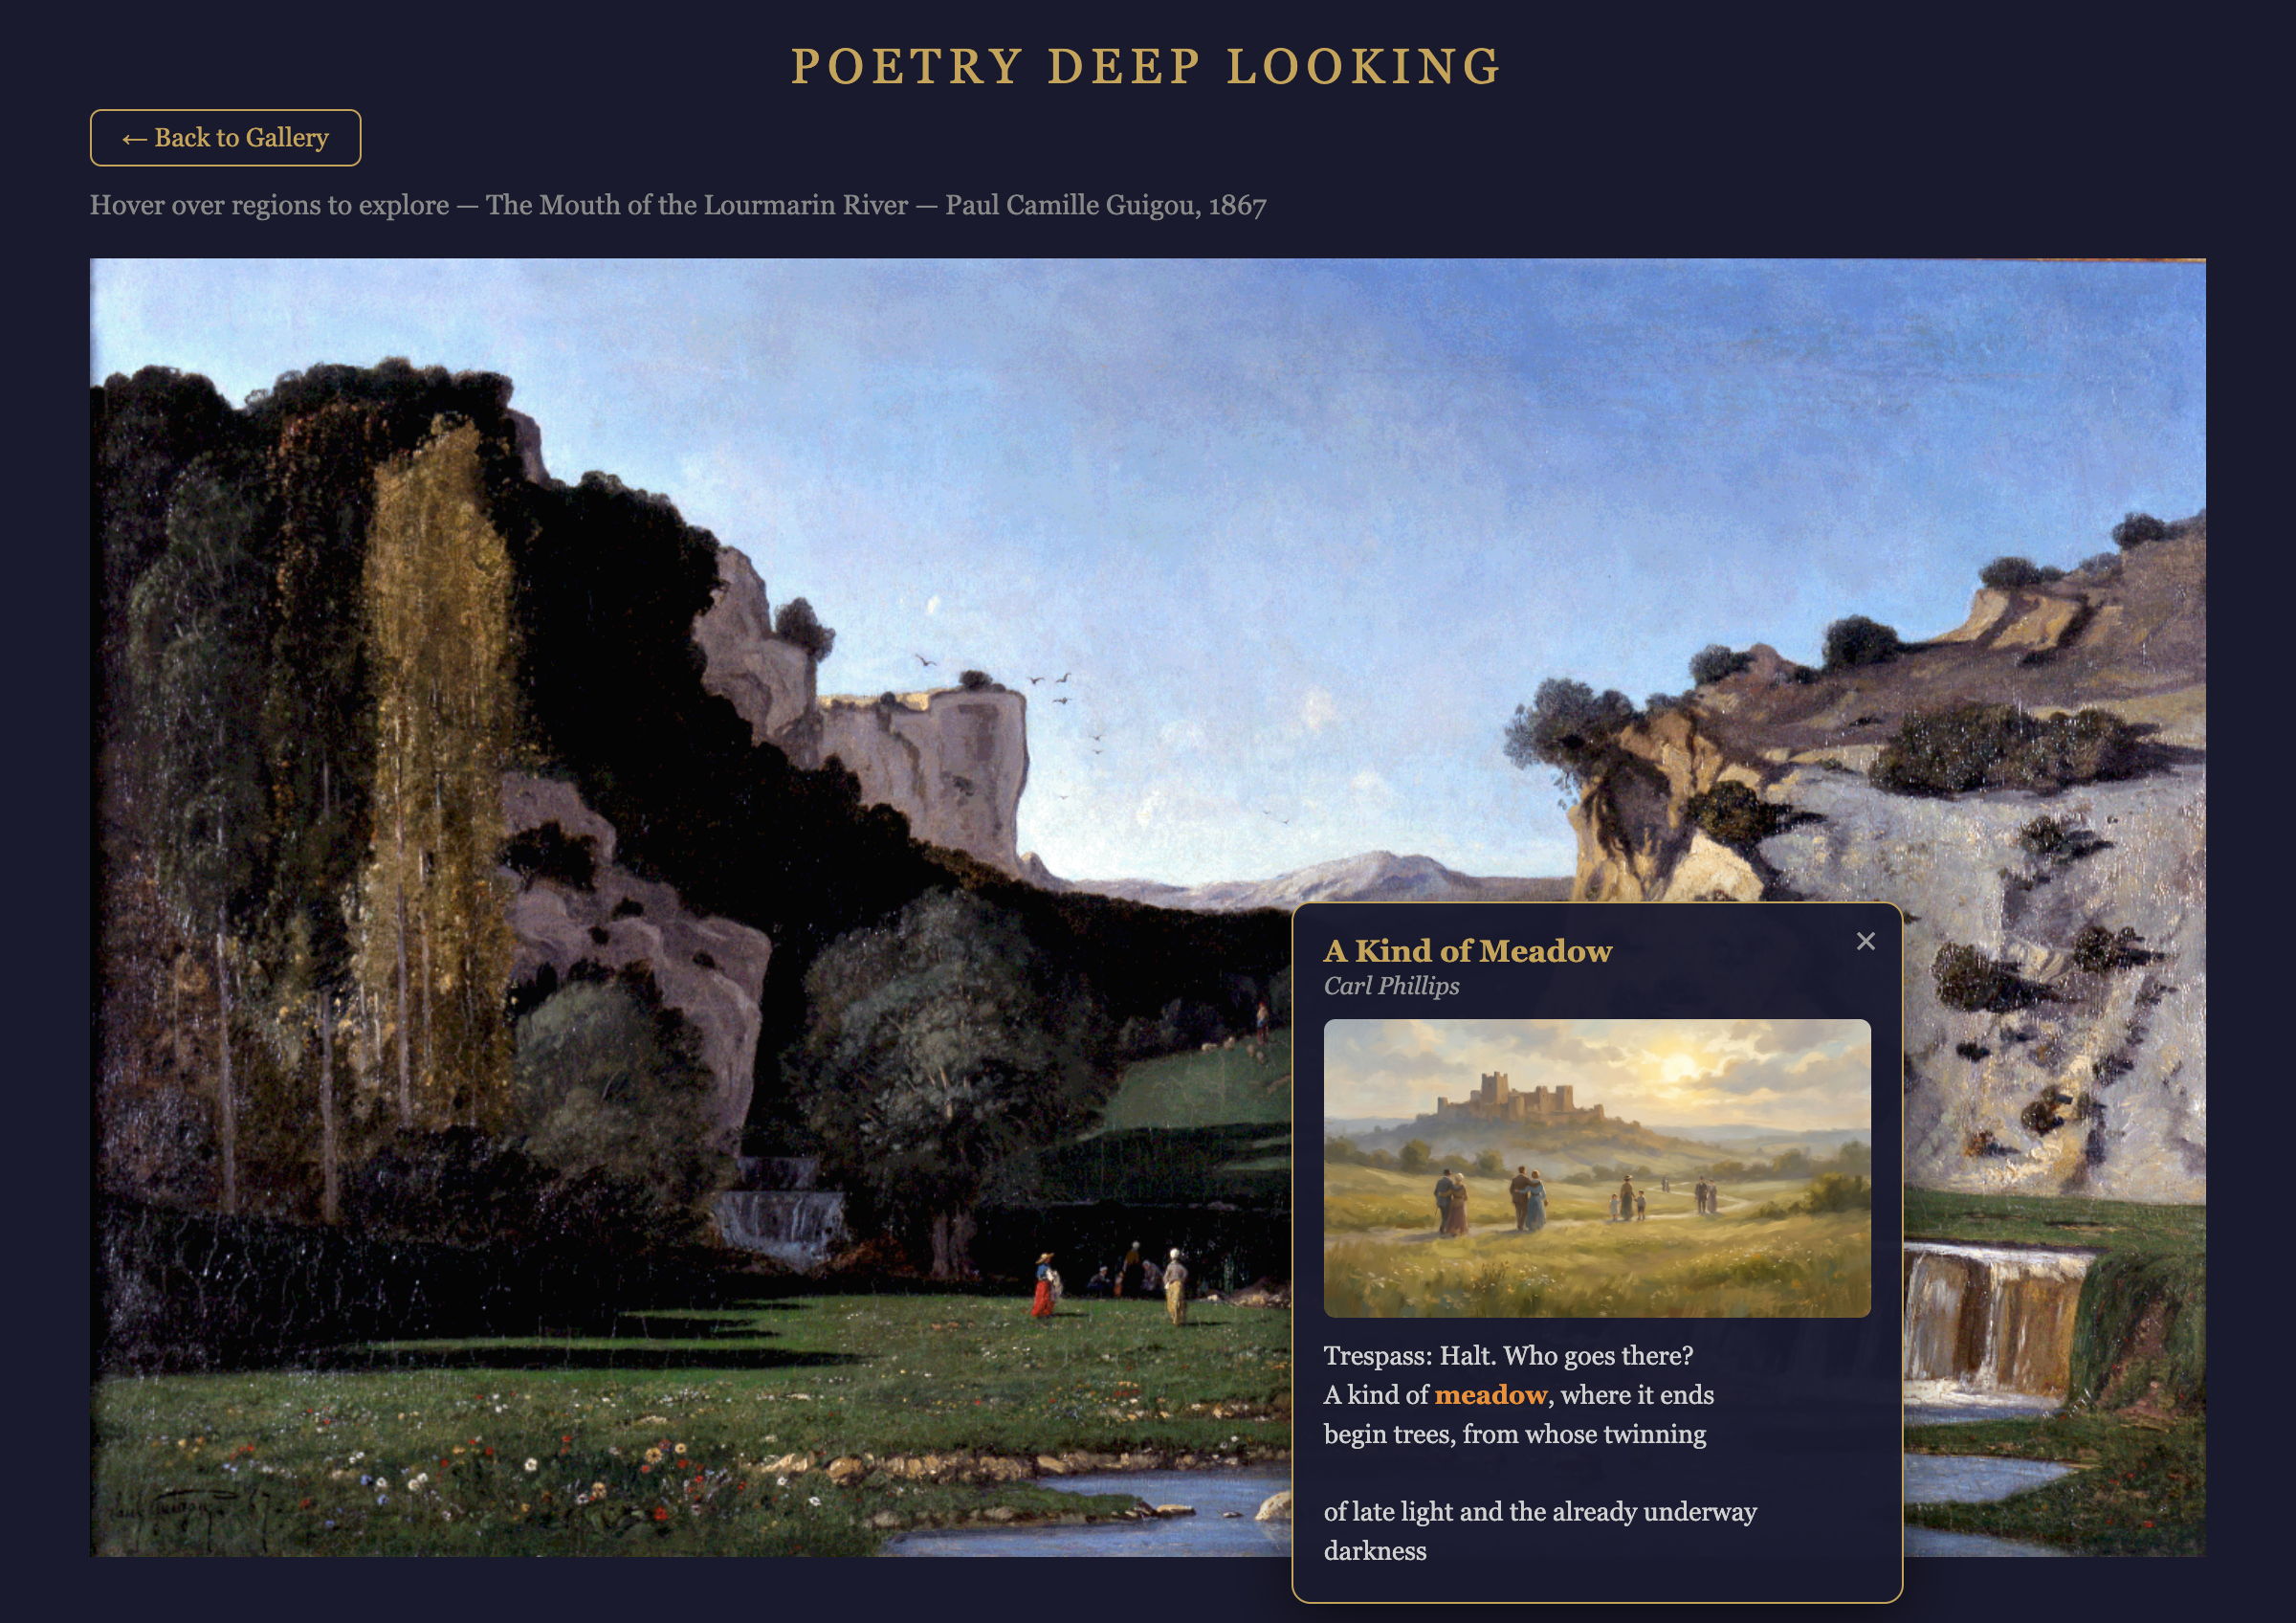
\includegraphics[width=0.85\textwidth]{lourmarin-pinned.png}
\caption{Pinned popup on the Lourmarin painting showing \emph{A Kind of Meadow} by Carl Phillips with the close button visible.}
\label{fig:lourmarin}
\end{figure}

\section{Technical Architecture}

The application is a single \texttt{index.html} file with embedded CSS and JavaScript:

\begin{itemize}
\item \textbf{Segmentation masks} are generated by Google Gemini Pro, producing flat-color region maps.
\item \textbf{Hover detection} uses pixel lookup on a hidden canvas --- no polygon data needed.
\item \textbf{Proportional coordinate mapping} handles the mismatch between displayed artwork size and mask dimensions.
\item \textbf{Poem data} is embedded as a JavaScript object, with each region mapped to a title, poet, excerpt, illustration, keyword, and URL.
\end{itemize}

\end{document}
